% !TEX root = ../KL-Projections.tex

%%%%%%%%%%%%%%%%%%%%%%%%%%%%%%%%%%%%%%%%%%%%%%%%%%%%%
\section{Multi-marginal  Optimal Transport}
\label{sec-multi-marginal}


Multi-marginal optimal transport is a natural extension of optimal transport with many 
potential fields of applications, see Section~\ref{sec-pw}. 


%%%%%%%%%%%%%%%%%%%%%%%%%%%%%%%%%%%%%%%%%%%%%%%%%%%%%
\subsection{Multi-marginal Regularization}
\label{subsec-multi-marginal-regularization} 
As in the barycenter problem, we are given $K$ marginals $(\km{p})_{k=1}^K$. 
We denote $\pi \in \RR_+^{N^K}$ a $K$-dimensional array, indexed as $\pi_j$ for $j=(j_1,\ldots,j_K) \in \{1\ldots,N\}^K$. 
The push-forward $S_k(\pi) \in \RR^N$ of such a $\pi$ along dimension $k$ is computed as
\eq{
	\foralls i \in \{1,\ldots,N\}, \quad
	S_k(\pi)_i \eqdef \sum_{j_1,j_2,\ldots,j_{k-1},j_{k+1}, ..,j_K}�\pi_{j_1,j_2,\ldots,j_{k-1},i,j_{k+1}, ..,j_K}.
}
The set of couplings between the marginals is
\eq{
	\Pi(p_1,p_2,\ldots,\km{p}) \eqdef 
	\enscond{ \pi \in \RR_+^{N^K} 
	}{ 
		\forall k, \quad S_k(\pi) = \km{p}
	}.
}

Given a cost matrix $C \in \RR_+^{N^K}$, the regularized OT problem~\eqref{eq-regul-transport} is generalized to this multi-marginal setting as
\eql{\label{eq-multimarg-entropic}
	\umin{\pi \in \Pi(p,q)} \dotp{C}{\pi} - \ga E(\pi).
}

Similarly as~\eqref{eq-regul-ot-kl}, this problem can be re-cast as a KL projection  
\eql{\label{eq-multimarginal-proj}
	\min_\pi \enscond{
		\KLdiv{\pi}{\xi} 
	}{
		\pi \in \Cc_1 \cap \Cc_2 \cap \ldots \cap \Cc_K
	}
	\qwhereq
	\xi \eqdef e^{-\frac{C}{\ga}}
}
where the exponentiation is exponent-wise, and where
\eq{
	\Cc_k \eqdef \enscond{ \pi \in \RR_+^{N^K} }{�S_k(\pi)=\km{p} }.
}

The Bregman projection on each of  the convex $\Cc_k$ are again given by a simple normalisation as detailed in the following proposition.

\begin{prop}
	For any $k$, denoting $\pi = \KLproj_{\Cc_k}(\bar{\pi})$, one has 
	\eq{
		\foralls j=(j_1,\ldots,j_K), \quad		
		\pi_{j} = \frac{(\km{p})_{j_k}}{ S_k(\bar\pi)_{j_k} } \bar\pi_{j}�
	}
\end{prop}

It is thus possible to use the Bregman iterative projection detailed in Section~\ref{sec-iterative-bregman} to compute the projection~\eqref{eq-multimarginal-proj}. 

We now detail in the two following sections two typical cases of application of multi-marginal OT: grid-free barycenter computation (Section~\ref{sec-multimarg-bary}) and resolution of generalized Euler flow (Section~\ref{sec-gen-euler}).

%%%%%%%%%%%%%%%%%%%%%%%%%%%%%%%%%%%%%%%%%%%%%%%%%%%%%
\subsection{Multi-marginal Barycenters}
\label{sec-multimarg-bary}

As shown in~\cite{Carlier_wasserstein_barycenter},�the computation of barycenters of measures (thus the continuous analogous of~\eqref{sec-barycenters}) can be computed by solving a multi-marginal transport problem. 

% \todo{Guillaume: I do not understand very clearly the point in this paragraph; is the goal  1) to solve the quadratic multi marginal OT by using the connection with the barycenter, 2) to solve the barycenter with multi marginal OT because it has the advantage of being grid-free or 3) check accuracy by comparing results between two methods}

% \todo{Gabriel: the goals are 2) and 3) (actually, not really checking accuracy, just visual comparison). An issue is to display the barycenter computed with multimarginal, since it is composed of lots of Diracs not on the grid. What Luca did is to re-introduce the grid, and do an histogramming (i.e. count the mass that falls in each bins) to obtain an image as displayed in the figure.  }


Let us suppose that the input measures $(\km{\mu})_{k=1}^K$ defined on $\RR^d$ are of the form $\km{\mu} = \sum_{i=1}^N p_{k,i} \de_{x_i}$, where $\km{p}=(p_{k,i})_{i=1}^N \in \Si_N$,  where $\{x_i\}_i \subset \RR^d$ and $\de_{x}$ is the Dirac measure at location $x \in \RR^d$. It is shown in~\cite{Carlier_wasserstein_barycenter} that the Wasserstein barycenter of the $\km{\mu}$ with weights $(\la_k)_k \in \Si_K$ for the quadratic Euclidean distance ground cost is 
\eql{\label{eq-continuous-barycenter}
	\mu_\la \eqdef \sum_{j=(j_1,j_2,\ldots,j_K)} % \pa{ \sum_k \la_k p_{k,j_k} }�
		 \pi_{j} \de_{ A_{j}(x)}%,\sum_k \la_k x_{j_k} }, 
}
% \todo{Guillaume: Sorry I do not understand this formula, it should depend on the optimal multi marginal coupling and I do not see it, that needs to be checked, also more user-friendly notations would be better   } 
% \todo{Gabriel: I modified the formula, it is ok now? What do you have in mind as new notations? The tricky point here is that we are discussing measure, whereas the remaining of the paper is dealing with histograms \ldots But it seems important to detail this formula with measure to explain how to shift from the multimarginal to barycenter. }
where $A_{j}(x)\eqdef \sum_k \la_k x_{j_k}$ is the Euclidean barycenter and $\pi \in \RR_+^{N^K}$ is an optimal multi-marginal coupling that solves~\eqref{eq-multimarg-entropic} for the following cost 
\eq{
	C_{j}  = \sum_{1 \leq k \leq K}\dfrac{\lambda_{k}}{2} \norm{ x_{j_k}-A_j(x) }^2.  % ,\, j_i \ne j_i'
}

An important point to note is that the measure barycenter~\eqref{eq-continuous-barycenter} is in general composed of more than $N$ Diracs, and that these Diracs are not constrained to be on the discretization grid $(x_i)_i$. In particular, the obtained result is different from the one obtained by solving~\eqref{eq-barycenter-regul}, which computes a barycenter that lies on the same grid as the input measures. In some sense, formulation~\eqref{eq-continuous-barycenter} is able to compute the ``true'' barycenter of measures, whereas~\eqref{eq-barycenter-regul} computes an approximation on a fixed grid, but the price to pay is the resolution of a high-dimensional multi-marginal program.  

Figure~\ref{fig:barm1} shows an histogram depiction of the measure $\mu_\la$ defined in~\eqref{eq-continuous-barycenter}, for the iso-barycenter (i.e. $\la_k=1/K$ for all $k$). It is computed by first solving~\eqref{eq-multimarg-entropic} with the same three marginals used in Figure~\ref{fig-barycenter-entropic}. The histogram $p \in \Si_N$ computed on a grid of $N=60 \times 60$ points. Each $p_i$ is the total mass of $\mu_\la$ in the discretization square $S_i$ of size $1/\sqrt{N} \times 1/\sqrt{N}$, i.e. $p_i = \mu_\la(S_i)$. 

%\todo{include simulation here}  

\begin{figure}[htdp]
	\centering
	\imgbox{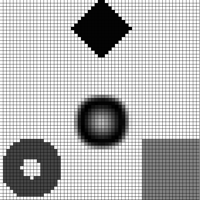
\includegraphics[width=.45\textwidth]{multimarginal/barMultimarginal}}
%		
	\caption{Barycenter computed by solving the multi-marginal problem with three marginals (annulus, diamond and square) discretized on an uniform 2-D grid of $N=60 \times 60$ points in $[0,1]^{2}$ and $\ga=0.005$. See the main text body for details about how the display of the barycenter measure is performed. }
  	\label{fig:barm1}
\end{figure} 


%%%%%%%%%%%%%%%%%%%%%%%%%%%%%%%%%%%%%%%%%%%%%%%%%%%%%
\subsection{Generalized Euler Flows}
\label{sec-gen-euler}

Brenier proposed in a series of papers~\cite{BrenierEulerAMS,BrenierEulerARMA,BrenierEulerCPAM} a relaxation of the Euler equation of incompressible fluids with constrained initial and  final data. 
These data are conveniently expressed as a volume preserving map $\Xi$ of the domain. This relaxation can be understood as requiring the resolution of a multi-marginal transportation   with an infinite number of marginals. Following~\cite{BrenierGeneralized} (equation (21) section VII), when discretizing this problem with $K$ steps in time, one thus faces the resolution of a $K$ marginals OT problem.
 

We consider a fixed uniform discretization of $[0,1]^d$ with points $(x_i)_{i=1}^N$. The marginals are the uniform measure on this set (as discretization of the Lebesgue measure), i.e. $\km{p}=\ones/N$ for all $k$. The prescribed volume preserving maps $\Xi : [0,1]^d \rightarrow [0,1]^d$ is discretized using a permutation of the grid points, i.e. a discrete bijection $\si : \{1,\ldots,N\} \rightarrow \{1,\ldots,N\}$.

The cost function is then
\eq{
	C_{j_1,\ldots,j_K}  = \sum_{k=1,\ldots,K-1} 
	\norm{ x_{j_{k+1}} - x_{j_{k}}  }^2   
	+  
	\norm{ x_{\si(j_1)} - x_{j_K} }^2 
}
and the optimal coupling $\pi$ solves~\eqref{eq-multimarg-entropic}.

For each $k \in \{1,\ldots,K\}$, the transition probability from "time"  $1$ to "time" $k$~: $T_{1,k} \in \RR^{N \times N}$ is defined as 
%\todo{Gabriel: I think there is a mistake in the formula bellow, $\sum_{j_i \ne {j_1,j_k}}$ should rather
%be $\sum_{j_2,\ldots,j_{k-1},j_{k+1},\ldots,j_K}$  I think.} 
\begin{equation}
\label{2coupl}
	\foralls (s,w) \in \{1,\ldots,N\}^2, \quad
	(T_{1,k})_{s,w} = \sum_{j_i \ne {j_1,j_k}} \pi_{s,j_2,\ldots,j_{k-1},w,j_{k+1},\ldots,j_K}.
\end{equation}
It represents the evolution of a generalized flow of particles at  time $t=\frac{k-1}{K-1}$.  Note that in this setting, particles trajectories are 
non deterministic and their mass may split and spread across the domain. 

%\todo{Guillaume: My understanding is that is a sort of transition probability between times $s$ and $t$ which should approach something concentrated on Lagrangian solutions whenever well defined? Anyway I think we should say clearly that having nondeterministic trajectories is well suited for Euler. Do you agree JD?}
%\todo{JD : Cant we just say that we recover Yann's results ... a refer to his paper ...} 

Brenier's numerical method~\cite{BrenierGeneralized} is based on an approximation of the measure preserving map by a one to one permutation of the domain and the representation of the diffuse coupling therefore needs a large number of particles. Our resolution method is different and computes a space discretization of the coupling matrix and naturally encodes non-diffeomorphic volume preserving maps. The coupling $\pi$ is an array of size $(N^d)^K$ where the $d$-dimensional physical domain is discretized on $N^d$ points and we have $K$ times steps. However, as explained in Remark~\ref{remjd} below, because of the structure of the cost we only need to store and multiply $(N^d)^2$ matrices. 
 
\begin{rem}\label{remjd}[Reduction to Transitions probabilities ]
As defined in~\eqref{eq-multimarginal-proj}, the resolution of the regularized $K$-marginal OT problem boils down to the computation of a KL projection of $\xi = e^{-\frac{C}{\ga}}$
We can rewrite the coupling using only 2 smaller matrices $\xi^0, \xi^1 \in \RR^{N \times N}$ since
\begin{equation}\label{gabarExp}
 	\xi_{j_{1},\ldots,j_{K}} = \pa{ \prod_{k=1}^{K-1} \xi^0_{j_{k},j_{k+1}} } \,  \xi^1_{j_{K}\si(j_{1})}
\end{equation}
\eq{
	\qwhereq
 	\xi^{0}_{\alpha,\beta} = 
	e^{-\frac{D_{\alpha \beta}}{\ga} },
	\quad\quad 
	\xi^{1}_{\beta,\alpha} = e^{-\frac{D_{\beta\si(\alpha)}}{\ga}}.
}
and $D_{\alpha \beta}=\norm{x_{\alpha}-x_{\beta} }^{2}$. 
%
We recall that all the marginals are equal to (a discretization of) the Lebesgue measure and $(x_{i})_i$ are discretized on the unit cube $[0,1]^{d}$.
As already noticed in Remark~\ref{rem-fast-sink},  the iterative Bregman projections~\eqref{eq-iter-bregmanproj} (always on the same Lebesgue marginal constraint)  can be simplified as an IPFP iterative procedure.
%
The optimal coupling $\pi$ that solves~\eqref{eq-multimarg-entropic} can be actually written as follows
\eq{
        \pi_{j_1,\ldots,j_K} = \xi_{j_1,\ldots,j_K} \prod_{k=1}^{K} u^k_{j_k} ,
}
where $u^k_{j_k}$ is the $(j_k)^{\text{th}}$ component of $u^k \in \RR^N$, for $k=1,\ldots,K$ (the $k^{\text{th}}$ vector being associated to the $k^{\text{th}}$ marginal).
Moreover the $u^k$ are uniquely determined by the constraints over the marginals of $\pi$
\eq{
   	u^k_{j_k} = \frac{1/N}{  
      	\sum_{m \neq k}  \sum_{j_m}  
		\{  \xi_{j_1,\ldots,j_K}   \prod_{\ell \neq k} u^\ell_{j_\ell}   \} 
	}
}
and the IPFP procedure for $K$ marginals is 
\eq{\label{IPFPmultimarg}
   u^{k,(n)}_{j_k} = \frac{1/N}{
   		\sum_{m \neq k} {\sum_{j_m}}  
		\{   \xi_{j_1,\ldots,j_K}  \prod_{\ell \neq k} {u^{\ell,(n-1)}_{j_\ell}}  \} 
	}
}
However, one can notice that the sum in~\eqref{IPFPmultimarg} could be computationally onerous, but thanks to~\eqref{gabarExp} we can rearrange it as   
\eq{
  	u^{k,(n)}_{j_k} =\frac{1/N}{ B_{j_k,j_k}}
}
where $u^{k,(n)}$ is the $k^{\text{th}}$ vector at step $(n)$ and $B$ is the the product of $K$ smaller $N \times N$ matrices 
\eq{
 	B=\xi^{\text{init}} \bigotimes_{\ell=1}^{K-1} \tilde{\xi}_{\ell}	
	\qwithq
	\xi^{\text{init}} = \choice{
		\xi^{0} \qforq k \neq K, \\
		\xi^{1} \quad \text{otherwise}
		}
}
\eq{
	\qandq
	\tilde{\xi}_{\ell} = \choice{
		\diag(u^{\sigma^k(\ell),(n)}) \otimes \xi^0 \qforq \sigma^k(\ell) \neq K \qandq \sigma^k(\ell) < k, \\
		\diag(u^{\sigma^k(\ell),(n-1)}) \otimes \xi^0 \qforq \sigma^k(\ell) \neq K \qandq \sigma^k(\ell) > k, \\
		\diag(u^{K,(n-1)})\otimes\xi^1 \quad \text{otherwise},
	}
}
%where the vectors \todo{are they vectors or matrices ? why $\RR^N \times \RR^N$ ? }�$\iter{u_i} \in \RR^N \times \RR^N$ satisfies $u_i^{(0)}=\ones$ and obey the recursion formula \todo{what does $b_j  \xi^0$ means (vector time matrix?) ?}
%\eq{
%	\iter{u_i}  =  
%	\frac{ 1/ n }{ \diag( \{ \prod_{j=1}^{K-1}   \diag(b_j  \xi^0 )\}    \diag({b_K} )  \xi^1    ) }  
%	\quad i = 1,\ldots,K 
%}
%\eq{	
%	\qwithq
%	b_j = \choice{
%		u_j^{(n-1)} \qforq j \neq i, \\
%		\ones \quad \text{otherwise}
%		}
%} 
%By a  slight abuse of notation $u_j^{(n-1)}$ is the latest update in the K loop (\todo{what does this mean?}�in a Gauss Seidel way). 
where $\otimes$ is the standard matrix product and we use the Matlab convention that $\diag$ of vector is the diagonal matrix with vector values and $\diag$ of matrix is the vector of its diagonal.
We also highlight that, to use the simplification the  %\todo{Gabriel: what does $u_{j\neq i}$ means ?}
 $u^l$ must be ordered in the correct way so that the computation of the sum for the  $k$ieth update starts at $k+1$ and finishes at $k-1$.
 We have introduced the circular  permutations $\sigma^{k}(\ell)=(\ell+k-1 \mod K)+1$ which 
returns the $(\sigma^k(\ell))^{\text{th}}$ term at the $\ell^{\text{th}}$ position of the product. 


Each iteration of the IPFP procedure therefore only involves $(2K)$ 2-coupling matrices multiplications and only requires 
storing $K$ vectors and the 2-coupling cost matrices  $\xi^0$ and  $\xi^1$. 
The computation of the 2-coupling maps \eqref{2coupl} can be simplified with the same remark. 
\end{rem}

Figures~\ref{fig:mm1}, \ref{fig:mm2} and~\ref{fig:mm3} show $T_{1,k}$ for three test cases in dimension $d=1$ proposed in~\cite{BrenierGeneralized}. The computation is performed with a uniform discretization $(x_i)_i$ of $[0,1]$ with $N=200$ points, $\ga=10^{-3}$ and $K=16$. They agree with the solutions produced by Brenier and the mass spreading of the generalized flow is nicely captured by the 2 marginals couplings~\eqref{2coupl}. 


\newcommand{\MyFigEuler}[2]{\imgbox{\includegraphics[width=.19\linewidth]{multimarginal/EulerT#1/EulerT#1timeStep#2}}}

\begin{figure}[h!]
	\centering
	\TabFive{
		\MyFigEuler{1}{1} &
		\MyFigEuler{1}{2} &
		\MyFigEuler{1}{3} &
		\MyFigEuler{1}{4} &
		\MyFigEuler{1}{5} \\
		$t=0$ & $t=1/8$ & $t=1/4$ & $t=3/8$ & $t=1/2$
	}
	\TabFour{
		\MyFigEuler{1}{6} &
		\MyFigEuler{1}{7} &
		\MyFigEuler{1}{8} &
		\MyFigEuler{1}{9} \\
		$t=5/8$ & $t=3/4$ & $t=7/8$ & $t=1$
	}
	\caption{% 
		Display of $T_{1,k}$ showing the evolution of the fluid particles from $x$ to $\Xi(x)=\min(2x,2-2x)$ for $x \in [0,1]$. The corresponding time is $t=\frac{k-1}{K-1} \in [0,1]$.
	}
   \label{fig:mm1}
\end{figure}


\begin{figure}[h!]
	\centering
		\TabFive{
		\MyFigEuler{2}{1} &
		\MyFigEuler{2}{2} &
		\MyFigEuler{2}{3} &
		\MyFigEuler{2}{4} &
		\MyFigEuler{2}{5} \\
		$t=0$ & $t=1/8$ & $t=1/4$ & $t=3/8$ & $t=1/2$
	}
	\TabFour{
		\MyFigEuler{2}{6} &
		\MyFigEuler{2}{7} &
		\MyFigEuler{2}{8} &
		\MyFigEuler{2}{9} \\
		$t=5/8$ & $t=3/4$ & $t=7/8$ & $t=1$
	}
	\caption{% 
		Same as Figure~\ref{fig:mm1} for the map $\Xi(x)=(x+1/2) \text{ mod } 1$ for $x\in [0,1]$. 
	}
   \label{fig:mm2}
\end{figure}



\begin{figure}[h!]
	\centering
		\TabFive{
		\MyFigEuler{3}{1} &
		\MyFigEuler{3}{2} &
		\MyFigEuler{3}{3} &
		\MyFigEuler{3}{4} &
		\MyFigEuler{3}{5} \\
		$t=0$ & $t=1/8$ & $t=1/4$ & $t=3/8$ & $t=1/2$
	}
	\TabFour{
		\MyFigEuler{3}{6} &
		\MyFigEuler{3}{7} &
		\MyFigEuler{3}{8} &
		\MyFigEuler{3}{9} \\
		$t=5/8$ & $t=3/4$ & $t=7/8$ & $t=1$
	}
	\caption{% 
		Same as Figure~\ref{fig:mm1} for the map $\Xi(x)=1-x$ for $x\in [0,1]$. 
	}
   \label{fig:mm3}
\end{figure}




    
